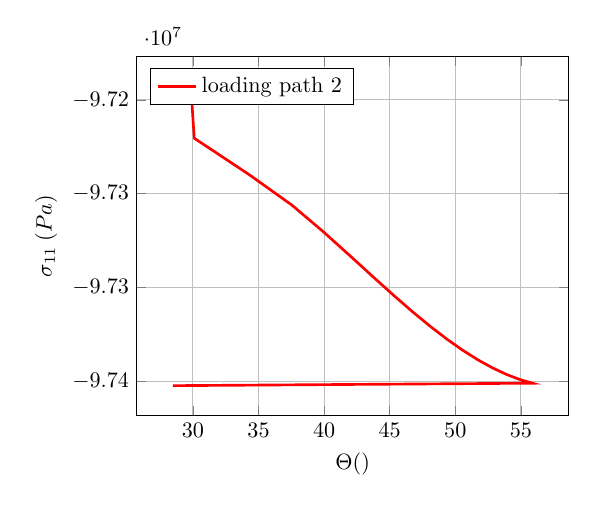
\begin{tikzpicture}[scale=0.8]
\begin{axis}[xlabel=$\Theta ()$,ylabel=$\sigma_{11} \: (Pa)$,ymajorgrids=true,xmajorgrids=true,legend pos= north west,title={}]
\addplot[Red,very thick,mark=none,solid] coordinates {(28.4635767022,-97402329.0528) (55.8871468593,-97401013.3503) (54.9098088796,-97399022.2449) (53.8970579746,-97396323.1292) (52.8447087528,-97392880.8127) (51.7476702341,-97388657.0297) (50.5996464827,-97383609.7965) (49.392696075,-97377692.5508) (48.1165591917,-97370852.963) (46.7575809036,-97363031.2297) (45.2968863803,-97354157.496) (43.707047502,-97344147.6953) (41.9453410294,-97332896.1792) (39.9379368574,-97320260.7129) (37.5326911321,-97306024.0872) (34.2661685833,-97289737.9866) (30.1003728946,-97270423.36) (29.9424332336,-97253779.6512) (29.9087413887,-97244122.3358) (29.9941747609,-97243007.9608) (29.9999183838,-97242992.0931) (29.9999988789,-97242991.8789) (29.9999999843,-97242991.8768) (29.9999999998,-97242991.8768) (30.0,-97242991.8768) (30.0,-97242991.8768) (30.0,-97242991.8768) (30.0,-97242991.8768) (30.0,-97242991.8768) (30.0,-97242991.8768) (30.0,-97242991.8768) (30.0,-97242991.8768) (30.0,-97242991.8768) (30.0,-97242991.8768) (30.0,-97242991.8768) (30.0,-97242991.8768) (30.0,-97242991.8768) (30.0,-97242991.8768) (30.0,-97242991.8768) (30.0,-97242991.8768) (30.0,-97242991.8768) (30.0,-97242991.8768) (30.0,-97242991.8768) (30.0,-97242991.8768) (30.0,-97242991.8768) (30.0,-97242991.8768) (30.0,-97242991.8768) (30.0,-97242991.8768) (30.0,-97242991.8768) (30.0,-97242991.8768) (30.0,-97242991.8768) (30.0,-97242991.8768) (30.0,-97242991.8768) (30.0,-97242991.8768) (30.0,-97242991.8768) (30.0,-97242991.8768) (30.0,-97242991.8768) (30.0,-97242991.8768) (30.0,-97242991.8768) (30.0,-97242991.8768) (30.0,-97242991.8768) (30.0,-97242991.8768) (30.0,-97242991.8768) (30.0,-97242991.8768) (30.0,-97242991.8768) (30.0,-97242991.8768) (30.0,-97242991.8768) (30.0,-97242991.8768) (30.0,-97242991.8768) (30.0,-97242991.8768) (30.0,-97242991.8768) (30.0,-97242991.8768) (30.0,-97242991.8768) (30.0,-97242991.8768) (30.0,-97242991.8768) (30.0,-97242991.8768) (30.0,-97242991.8768) (30.0,-97242991.8768) (30.0,-97242991.8768) (30.0,-97242991.8768) (30.0,-97242991.8768) (30.0,-97242991.8768) (30.0,-97242991.8768) (30.0,-97242991.8768) (30.0,-97242991.8768) (30.0,-97242991.8768) (30.0,-97242991.8768) (30.0,-97242991.8768) (30.0,-97242991.8768) (30.0,-97242991.8768) (30.0,-97242991.8768) (30.0,-97242991.8768) (30.0,-97242991.8768) (30.0,-97242991.8768) (30.0,-97242991.8768) (30.0,-97242991.8768) (30.0,-97242991.8768) (30.0,-97242991.8768) (30.0,-97242991.8768) (30.0,-97242991.8768) };
\legend{loading path 2}
\end{axis}
\end{tikzpicture}
%%% Local Variables:
%%% mode: latex
%%% TeX-master: "../../mainManuscript"
%%% End:
